\section{HBase}

%\cite{Redt01} embeddeed in text.
%\cite{SpaOd16} embeddeed in text.


Im Folgenden wird HBase als die Hadoop Datenbank vorgestellt, die zu Grunde liegende Systemtechnologie erläutert  und die Installation/Konfiguration beschrieben.
\subsection{Visitenkarte}
\subsubsection{Entstehung}
Nachdem Google immer größer werdende Datenmassen speichern musste und dieses Problem mit dem  \ac{GFS} gelöst zu sein schien, stellten sich weitere Probleme heraus: 
Die Indexierung dieser Daten und die Verteilung der Daten auf viele Knoten ohne Zugriffgeschwindigkeit und Konsistenz zu verlieren. Google fand eine Lösung mit BigTable und auf Grundlage des veröffentlichten WhitePapers \cite{bigtable} dazu, entwickelte die Open-Source-Community dann HBase. Aus diesem Grund weisen diese beiden Datenbanken auch Gemeinsamkeiten bezüglich ihrer Funktionalität auf. Beispielsweise unterstützen beide die Komprimierung (siehe \ref{komprimierung}) und Versionierung der Daten.

\subsubsection{Allgemein}
HBase wurde entwickelt, um mit Hadoop zusammen zu arbeiten und ist ein verteiltes BigData-Speichersystem für strukturierte Daten. 
%TODO was heißt strukturiert ?
 und bietet einen schnellen (nahe Echtzeit) Zugriff auf riesige Datenmengen. In HBase lassen sich diese Datenmengen auf mehreren Knoten verteilen, verwalten und jederzeit erweitern. HBase basiert auf Java, ist Open-Source, nicht-relational, spaltenorientiert und setzt auf ein verteiltes Dateisystem wie HDFS von Hadoop auf. HBase als Key-Value-Store wurde als fehlertolerantes System entworfen, das auch unvollständige Datenmengen zu speichern weiß. Durch \ac{WAL} und eine verteilte Konfiguration kann sich HBase schnell von Serverausfällen erholen \cite{Redt01}. Nach CAP-Theorem legt es besonders Wert auf Verfügbarkeit und Partitionierung und vernachlässigt die Konsistenz der Daten. Des weiteren unterstützt HBase die Replikation von Hadoop, den MapReduce-Algorithmus, automatische Verteilung der Tabellen auf die Knoten, automatische Verteilung der Last, Komprimierung der Daten und Bloom-Filter. HBase kann im Standalone-Modus, im pseudo-verteilten Modus und im vollständig-verteilten Modus betrieben werden. Für den vorliegenden Usecase wird am Ende des Kapitels die Konfiguration für den vollständig-verteilten Modus beschrieben. Für diesen Modus wird für die verteilte Konfiguration ein Zookeeper benötigt. HBase stellt zwar selbst keine SQL-API zur Verfügung lässt sich aber durch Schnittstellen wie Apache Phoenix um eben solche erweitern.

%Bei unvollständigen Datensätzen, im Relationalen Sinne gesprochen, bei Einträgen mit fehlenden Attributen und einem sich oft wechselndem Schema empfiehlt sich der Einsatz von HBase.
%speicherbasierte Tabellen
%Bietet geringe Latenz bei Zugriff auf kleine Teil-Datenmengen 
%Bietet ein flexibles Datenmodel
%build for low latency querries
%Ein verteiltes Speichersystem für strukturierte Daten

%Key-value
%value wird von einem Key identifiziert
%Key und value sind beide byte-array
%Werte können schnell durch die Schlüssel zugegriffen werden

\subsubsection{Portfolio}
HBase wird von vielen bekannten Konzernen eingesetzt, da es sich gut für Logging- und Suchsysteme  eignet und als Grundpfeiler für \ac{OLAP}-Systeme glänzt \cite{Redt01}.

\begin{figure}[htbp] 
  \centering
     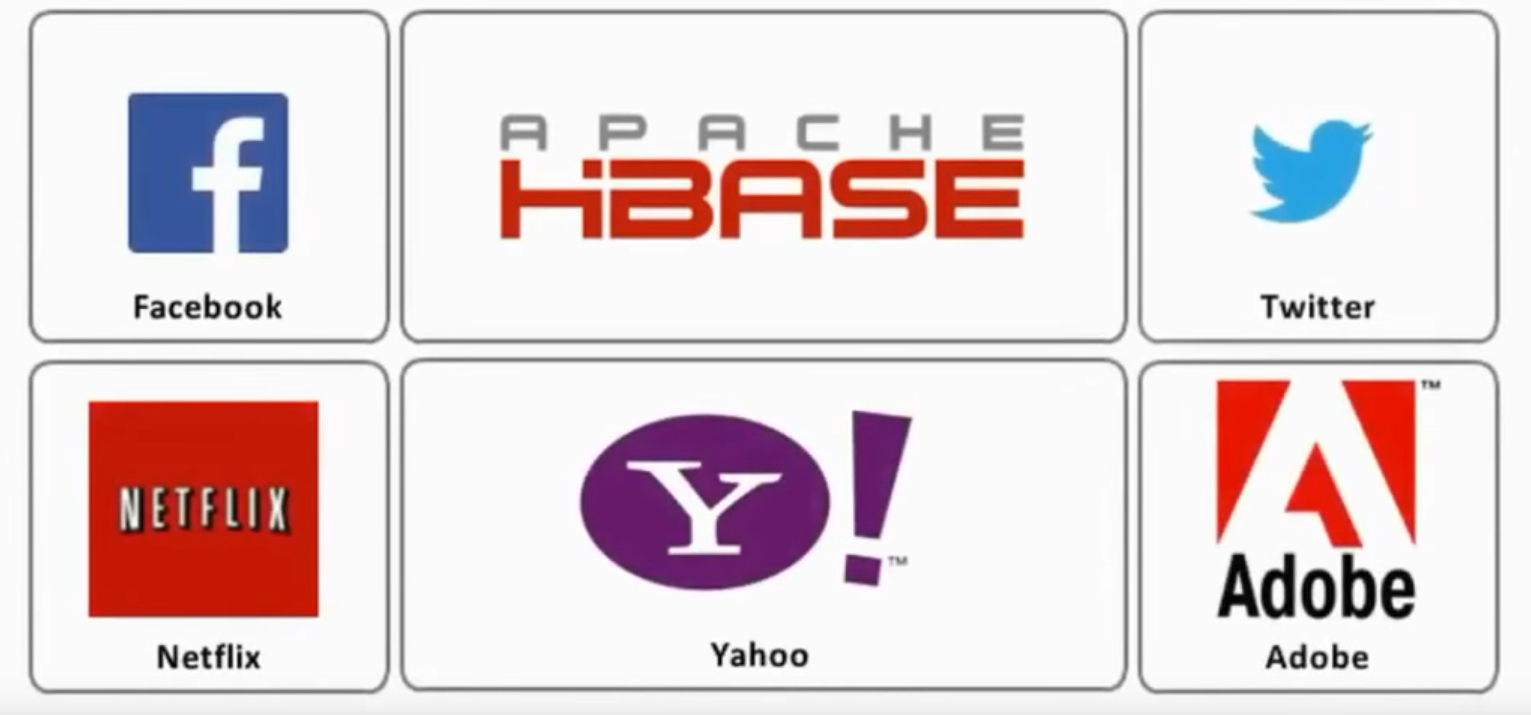
\includegraphics[width=0.7\textwidth]{images/portfolio.png}
  \caption{HBase-Portfolio}
  \label{fig:Portfolio}
\end{figure}

\subsection{Systemtechnologie} % ausgewählte technologische Aspekte (Architektur, Funktionsweise, ...) ohne (ausführliche) Modellierungsaspekte

\subsubsection{Hbase im Vergleich zu einem relationalen Datenbank-Managementsystem}
HBase erinnert an eine relationale Datenbank, da die Daten in Tabellen gespeichert werden, die Zellen enthalten. Jedoch verhalten sich die Tabellen nicht wie Relationen und die Zeilen nicht wie Datensätze in relationalen Datenbanken. Auch sind die Spalten nicht durch ein Schema definiert.
HBase speichert die teils unvollständigen Daten in Spalten ab im Vergleich zu vollständigen Reiheneinträgen in einem RDBMS. Dies ist notwendig da große Datenmengen den Anforderungen auf Vollständigkeit, wie sie ein RDBMS erfordert, oftmals nicht gerecht werden.  
Während in einem RDBMS viele schmale, normalisierte Tabellen vorliegen, ist HBase für Tabellen mit Millionen von nicht-normalisierrten Spalten ausgelegt. Die Partitionierung wird bei HBase automatisch vogenommen, währenddessen in einem RDBMS dies manuell erfolgen muss.


\subsubsection{HBase im Vergleich zu HDFS}
Das \ac{HDFS} ist ein Dateisystem für das Abspeichern von Daten auf Clustersystemen. Im Unterschied zu normalen Dateisystemen wie ext4 oder NTFS kümmert es sich automatisch um die Replikation von Daten zwischen den Knoten,  
sodass eine hohe Skalierbarkeit und eine hohe Ausfallsicherheit entsteht. Zudem ermöglicht das einen schnellen, parallelen Zugang für die Anwendungen von MapReduce. Da HDFS ein Filesystem ist, fehlt ihm die zufällige Lese-und Schreibfähigkeit. Eine mögliche Lösung dafür ist HBase. Es stellt innerhalb des Clusters in Echtzeit Lese- und Schreibzugriff zu den Daten her. HBase ist besonders nützlich, wenn es um die Verarbeitung von sehr großen Datenmengen geht. Es wird empfohlen HBase in einem verteilten System ab fünf Knoten einzusetzen.

%TODO: Architektur-Grafik

\subsubsection{Master-Slave-System}
HBase besitzt zwei Rollen: den HBase Master Server und die RegionServer.

\subsubsection{Master Server}
Der Master Server ist verantwortlich für die Zuweisung der Regionen an die RegionServer, die Verteilung der Last (Link), den Neustart der RegionServer, die Teilung (Link) und das Überwachen der RegionServer. Es ist möglich mehrere Master in einem Cluster zu betreiben, wobei aber nur einer aktiv sein kann. Da der Master nur verwaltende Funktionen inne hält, kann ein Cluster auch ohne Master Server arbeiten, solange kein RegionServer ausfällt. Spätestens dann muss der Master Server eingreifen und die Regionen neu zuweisen. Die Verfügbarkeit des Masters wird vom Zookeeper verwaltet.

\subsubsection{RegionServer}
Der RegionServer beinhaltet die HBase Regionen (siehe \ref{region}) und die HBase-Daten. Die Aufrufe der JAVA-API gehen direkt an den RegionServer, damit der Master Server nicht als Flaschenhals agiert. Der RegionServer komprimiert und verteilt die Daten und berichtet dem Master Server. Es wird empfohlen nur einen RegionServer pro Maschine zu betreiben \cite{Redt01}. Für Lese-und Schreibzugriffe kommuniziert der RegionServer mit anderen RegionServern.
%Halten Tabellen, lesen und puffern Schreibzugriffe

\subsection{Datenmodell} %Modellierungsaspekte
\subsubsection{Tabellen}
HBase speichert die Daten, ähnlich wie eine relationale Datenbank in Tabellen. Jedoch bestehen diese aus Reihenschlüsseln und Spaltenfamilien (siehe \ref{sf}). Es gibt zwei Arten von Tabellen: Die Benutzer-Tabellen und die System-Tabellen.
Die Systemtabellen werden für das Verwalten von \acp{ACL}, Meta-Daten für die Tabellen, Regionen (siehe \ref{region}) und Namensräumen verwendet. Die Benutzer-Tabellen werden im vorliegenden Usecase für die Verwaltung des Million-Song-Dataset verwendet. Folgend ein Beispiel einer solchen Tabelle:

\begin{figure}[htbp] 
  \centering
     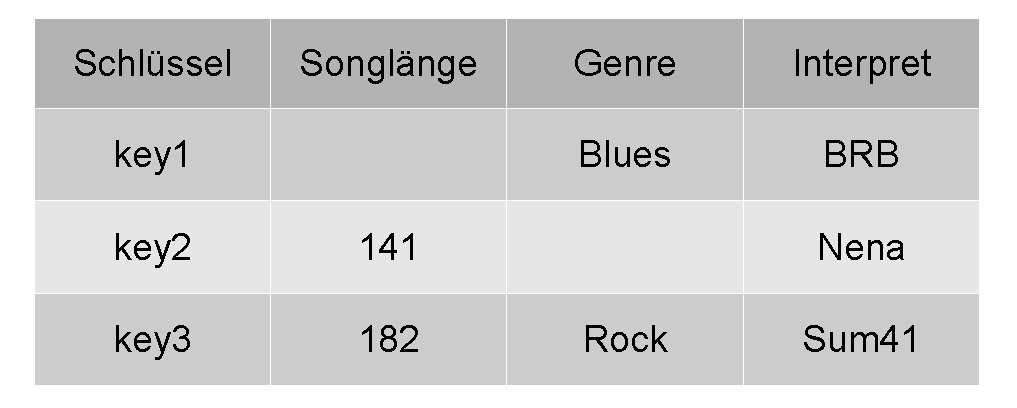
\includegraphics[width=0.7\textwidth]{images/logisch.pdf}
  \caption{Logische Darstellung der Daten}
  \label{fig:Logische Darstellung der Daten}
\end{figure}

%Tablellen sind nach Reihen-schlüssel sortiert


\subsubsection{Regionen}\label{region}
Eine Tabelle besteht aus Spalten und Reihen. Für die Skalierung  und den randomisierten Zugriff, teilt HBase die Tabelle horizontal in Regionen auf, d.h. jede Region besteht aus einer Reihe von aufeinander folgenden Schlüsseln. Jede Region wird einem RegionServer zugeordnet. Der HBase LoadBalancer sorgt dafür, dass die Regionen auf alle RegionServer gleich verteilt werden. Jede Region wird durch einen Start-Schlüssel und einen End-Schlüssel begrenzt. Diese Informationen lassen sich in den System-Tabellen wiederfinden. Regionen können geteilt werden, wenn sie zu groß werden oder zusammengelegt werden, wenn die zu klein sind.

\subsubsection{Spaltenfamilien}\label{sf}
Die Vorgabe ist, dass Daten mit gleichen Zugriffs-Queries und dem selben Format in einer Spaltenfamilie zusammengefasst werden sollten. Wenn wir beispielsweise zu allen Songs des One-Million-Song-Datasets die Cover der CDs hinterlegt hätten, könnten die Bilder in einer Spaltenfamilie und die textuellen Informationen zu den Songs in einer anderen Spaltenfamilie hinterlegt werden. So könnte die Spaltenfamilie mit den textuellen Informationen komprimiert werden. Oder wenn bestimmte Daten nur gelesen werden und andere meistens geschrieben werden, sollte über eine zweite Spaltenfamilie nachgedacht werden. Es gibt keine Grenze nach oben für die Spaltenfamilien innerhalb einer Tabelle, jedoch leidet die Performanz bei vielen Spaltenfamilien. Der MemStore (siehe \ref{memstore} wird belastet und generiert viele kleine Dateien. Bei der Tabellenerzeugung  muss bis auf die Spaltenfamilien keine feste Vorgabe gemacht werden. Alles außer der Tabellenname wird als Byte-Array abgespeichert, d.h. man kann Zeichen, Zahlen, Buchstaben usw. abspeichern. Um auf einen Wert zugreifen zu können, muss der Reihenschlüssel, die Spaltenfamilie, der Spaltenname und ein Zeitstempel angegeben werden.

\begin{figure}[htbp] 
  \centering
     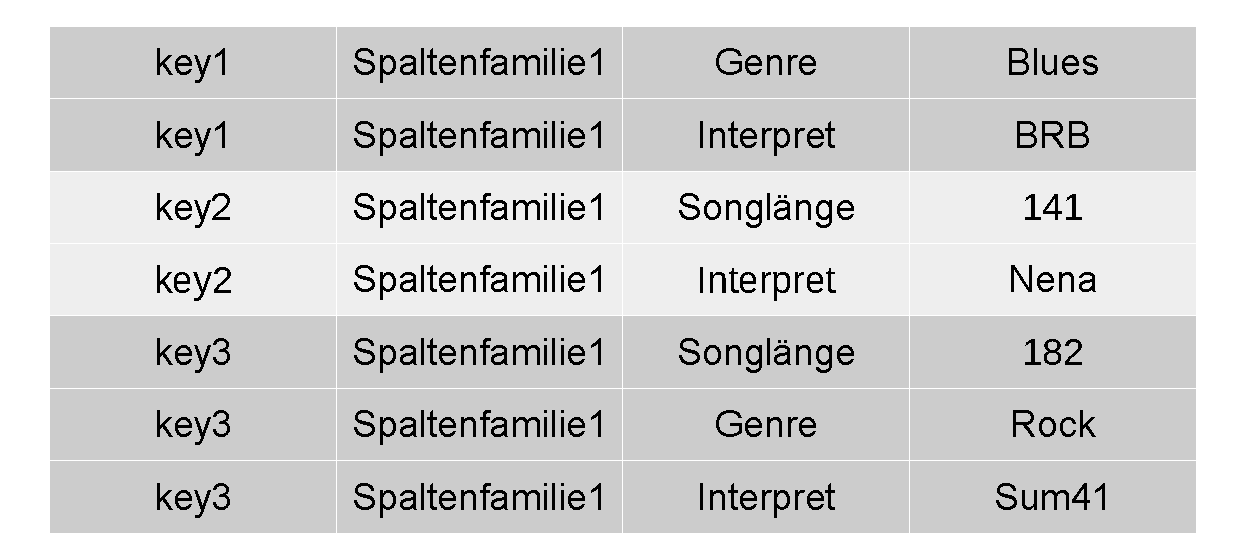
\includegraphics[width=0.7\textwidth]{images/physisch.pdf}
  \caption{Physische Darstellung einer Tabelle}
  \label{fig:Physische Darstellung einer Tabelle}
\end{figure}


%Wie in der Abbildung zu sehen ist, werden alle Spalten zusammen in einer Reihe abgespeichert. Beim Hinzufügen einer Reihe wird sie in den Commit-Log geschrieben, bevor dieser im den MemStore gelegt wird.

\subsubsection{Spalten}
Spalten werden nicht durch eine Schema-Beschreibung vorgegeben und können jederzeit zu einer Spaltenfamilie hinzugefügt werden. Jede Spalte kann mehrere Versionen erhalten. 

\subsubsection{Stores}
Es gibt einen Store pro Spaltenfamilie. Ein Store gruppiert den MemStore und 0-x MemStore-Files (HFiles). Diese Datei beinhaltet alle Informationen, die in die Tabelle hineingeschrieben und herausgelesen werden.

\subsubsection{MemStore}\label{memstore}
Wenn Daten hinzugefügt werden, wird ein \ac{WAL} erzeugt und in den MemStore gelegt. Der MemStore wird periodisch ins HDFS geflusht. Alle Updates und Lese-Operationen werden vom MemStore vorgenommen.

\subsubsection{HFiles}
HFiles (Key-Value-Map) werden erzeugt, wenn die MemStores voll sind und werden im HDFS abgespeichert, um von der Hadoop-Persistierung und Replikation zu profitieren. HFiles bestehen aus Blöcken. Ein Block hat eine Größe zwischen 8KB und 1 MB. Die Blockgröße kann konfiguriert werden.  Die Standard-Größe liegt bei 64KB. Es gibt viele Blocktypen die innerhalb eines HFiles vorkommen können: Der Datenblock enthält sowohl die Daten als auch die \textit{Put- und Delete-Markierungen}. Indexblocks ermöglichen das schnelle Auffinden einer Reihe innerhalb eines HFiles. Bloom-Filter-Blocks werden für das Überspringen von  bestimmten Parse-Vorgängen genutzt, damit der angefragte Schlüssel schneller gefunden werden kann. Trailer Blocks enthalten die HFile-Version. 
%HFiles sind unveränderlich, da HDFS kein Update erlaubt.
Zusammenfassende eine Darstellung der HBase-Architektur:

\begin{figure}[htbp] 
  \centering
     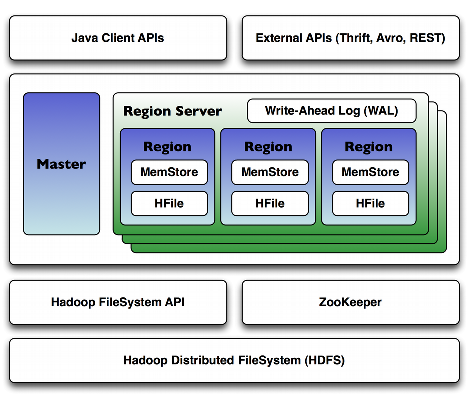
\includegraphics[width=0.7\textwidth]{images/architecture.pdf}
  \caption{HBase-Architektur}
  \label{fig:HBase-Architektur}
\end{figure}



\subsubsection{Interne Tabellenoperationen}
Die große Stärke von HBase ist es, Daten zu größeren Dateien zusammenzufassen und Tabellen auf mehrere Server zu verteilen. Hierzu verwendet HBase drei verschiedene Mechanismen.

\subsubsection{Komprimierung}\label{komprimierung}
HBase speichert alle Operationen im MemStore ab. Falls dieser voll ist werden die HFiles in das Filesystem geschrieben. Um zu vermeiden, dass viele kleine HFiles entstehen, verdichtet HBase sie zu größeren Dateien. Beim Löschen von Zellen setzt HBase einen Marker, der bei der Verdichtung überprüft wird. Alle Dateien mit dem gleichen Schlüssel, aber einem älteren Zeitstempel werden so gelöscht. In einer weiteren Stufe der Verdichtung können alle Marker gelöscht werden. Eine solche Verdichtung kann manuell für eine spezifische Region oder Tabelle angestoßen werden. Außerdem werden standardmäßig wöchentlich solche Verdichtungen von HBase selbst ausgeführt.

\subsubsection{Teilung}
Das Gegenteil der Verdichtungen ist die Teilung (Split), auch Auto-Sharding genannt. Wenn eine Region eine Größe von 10GB erreicht, führt HBase eine Teilung durch und es entstehen zwei neue Regionen. Hierbei ist zu beachten, dass Teilungen immer spaltenfamilienübergreifend stattfinden:

\begin{figure}[htbp] 
  \centering
     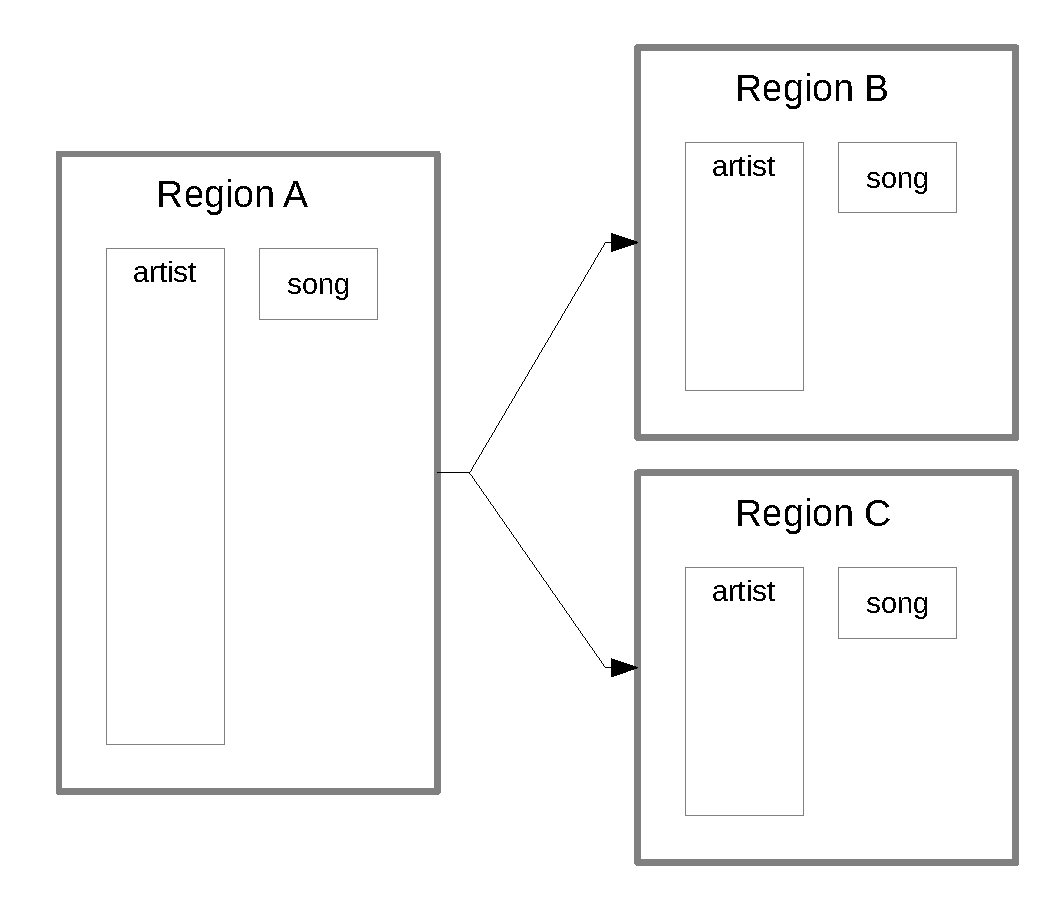
\includegraphics[width=0.7\textwidth]{images/split.pdf}
  \caption{Zwei Spaltenfamilien nach vor und nach der Teilung}
  \label{fig:Teilung}
\end{figure}


\subsubsection{Verteilung der Last}
Eine Verteilung der Last ist insbesondere bei der Neuordnung von Daten (Komprimierung) oder der Veränderung der Cluster-Umgebung (neue oder entfernte Rechnerknoten) notwendig.
%Da Regionen geteilt und verdichtet werden, neue Server hinzukommen oder herunterfahren ist eine Balancierung der Last notwendig.
HBase führt alle fünf Minuten einen LoadBalancer aus der algorithmisch sicherstellt, dass alle RegionServer eine ähnliche Anzahl an Regionen bedienen. 

 \subsubsection{Versionierung}
Eine Reihe, eine Spalte und ein Zeitstempel spezifizieren exakt eine Zelle in HBase. Während Spalten und Reihen gleich bleiben können, ändert sich der Zeitstempel für jede Zelle. Der Zeitstempel, als Long-Integer-Datentyp, wird in absteigender Reihenfolge hinterlegt, sodass immer der aktuellste Wert aus den HFiles gelesen wird \cite{reference}.


\subsubsection{Zugriff auf HBase}
Obwohl aus Perfomanzgründen empfohlen wird die JAVA-API für den Zugriff auf HBase zu nutzen, werden im folgenden weitere Möglichkeiten vorgestellt.

\subsubsection{Thrift Server}
Der Thrift Server kann als Gateway benutzt werden, um Applikationen  anderer Sprachen, den Zugriff auf HBase zu ermöglichen. Ein C/C++ Client könnte bei dieser Lösung jedoch nur mit dem Thrift Server kommunizieren und nicht direkt auf einen RegionServer zugreifen.

\subsubsection{REST Server}
HBase stellt auch eine REST-API zur Verfügung, auf die über HTTP zugegriffen werden kann.

%\subsubsection{Avro}


\subsection{Systeminstallation} %Installation auf der Grundlage unseres Clusters 
Für die Installation werden sowohl auf dem Master Server als auch auf den RegionServern folgende UNIX-Kommandos abgesetzt:
\noindent 
\begin{lstlisting}[language=bash]
  $ wget http://www-us.apache.org/dist/hbase/stable/
    hbase-1.2.4-bin.tar.gz
  $ tar -xzf hbase-1.2.4-bin.tar.gz
  $ ln -s hbase-1.2.4 hbase
  $ cd hbase
  $ export PATH=$PATH:~/hbase/bin
\end{lstlisting}

Die Konfiguration für HBase wird in einer Datei namens \textit{hbase-site.xml} erstellt. Hier werden Zookeeper-Einstellungen vorgenommen, das HDFS-System referenziert und der Betriebsmodus sowie der Pfad zur Datenspeicherung eingestellt.
Um HBase zu starten, wird der Befehl 
\noindent 
\begin{lstlisting}[language=bash]
  $ {HBASE_HOME}/bin/start-hbase.sh 
\end{lstlisting}
ausgeführt. HBase lässt sich mit dem Standard-Port 16010 über folgende \ac{URL} über die Weboberfläche aufrufen: \textit{localhost:16010}

\subsubsection{ZooKeeper}
ZooKeeper ist ein Open-Source-Projekt unter der Apache-Foundation. ZooKeeper wird auf den Knoten von Clustern installiert und bietet 
Dienste für typischen Aufgaben an, die bei verteilten Anwendungen auf Clustern anfallen. Typische Probleme sind dabei Race-Conditions 
beim verteilten Schreiben auf den selben Daten, der Zugriff auf schon veraltete Daten oder überhaupt das Auffinden von den Rechnerknoten im
Cluster. ZooKeeper überwacht auch die einzelnen Knoten im Cluster durch sogenannte \textit{Heartbeats}. Dies sind kurze Signale an den Master,
die signalisieren, dass der Rechnerknoten noch aktiv ist. 

Die Installation von ZooKeeper ist verhältnismäßig einfach. Nachdem die Anwendung auf die einzelnen Knoten herunter geladen ist, muss in der 
\newline \texttt{zookeeper/conf/zoo.cfg}
die Konfiguration erfolgen, die im einfachsten Falle nur aus der Angabe der Rechner-Knoten besteht. Innerhalb von ZooKeeper nennt sich so ein Verbund
von Rechner-Knoten ein \textit{esemble}. Diese Konfiguration muss anschließend auf alle Knoten verteilt werden. Danach kann der ZooKeeper-Server, genannt \texttt{zkServer},
auf jedem Knoten manuell gestartet werden. Über den Client-Port von ZooKeeper, der in diesem Projekt auf jedem Knoten der Port $2186$ ist, können die verteilten
Anwendungen die ZooKeeper-API verwenden. Dabei können sie sogenannte \textit{zNodes} anlegen. Das sind Dateien, auf die verteilt zugegriffen wird und um dessen
Gültigkeit sich nun ZooKeeper kümmert, sodass die verteilte Anwendung sich nicht mehr um die typischen Probleme, die in einem Cluster auftauchen, kümmern muss.

\subsection{Datenschema}\label{hbase_datenschema}
\subsection{Ad-Hoc-Zugriffsmöglichkeiten}\label{hbase_adhoc}